\chapter{Conclusiones y líneas futuras}
\label{cap:discusion_conclusiones}

Como punto final al trabajo técnico realizado durante este proyecto   
se procede a revisar todos los objetivos de mayor y menor nivel planteados al inicio del mismo. A continuación se valoran las ventajas y limitaciones observadas durante la ejecución del proyecto, así como se discute la conveniencia de las soluciones adoptadas. Por último se extrae un conjunto de conclusiones generales del trabajo realizado, indicando posibles lineas futuras de trabajo.

\section{Conclusiones de objetivos funcionales}
En esta sección se realiza una revisión de los objetivos planteados en el capítulo \ref{cap: objetivos}. Como objetivo principal se propuso la implementación de una arquitectura de control basada en ROS2 para que se pueda operar de forma sencilla la fase de preparación de una estación robotizada de fabricación aditiva no planar. 

Al tratarse de un enfoque amplio en el que se tocaban diferentes áreas de robótica industrial se procedió a establecer cuatro objetivos secundarios: Diseño de arquitectura de control, elaboración de un sistema de toma de datos del manipulador robótico, implementación de un algoritmo de trazado de trayectorias a partir de modelos \acrshort{CAD} y desarrollar un controlador sencillo que permita calentar y regular de forma automática la plataforma de impresión. 

En las siguientes líneas se revisa que cada objetivo propuesto se haya completado y se indican algunos aspectos destacados de cada paquete de trabajo.

\begin{itemize}
    \item En cuanto al diseño de la arquitectura de control (capítulo \ref{cap: diseno_arquitectura}):
    \begin{enumerate}
        \item Se ha definido una lista de especificaciones y funcionalidades generales que debe cumplir la estación robotizada.
        \item Se ha establecido el alcance de cada sección del marco de trabajo, indicando sus principales necesidades. Además, se describe el tipo de comunicaciones entre cada cada sección que pueden ser de utilidad e interés común para el resto de agentes involucrados.
        \item Se ha hecho un estudio de los flujos de trabajo con mayor impacto en la literatura. Posteriormente se ha definido uno característico para la estación del proyecto, dejando claramente separadas las diferentes fases y etapas que lo componen.
        \item Se han identificado los actores esenciales de una arquitectura de control y comunicaciones de una estación robotizada de fabricación. Con este información se ha diseñado una arquitectura propia de control adaptada al flujo de trabajo elaborado anteriormente. De este modo también se especifica el tipo, funcionalidad, contenido y elementos implicados en cada mensaje y bloque de control.
    \end{enumerate}

    \item En cuanto al sistema de lectura de datos del cobot (capítulo \ref{cap:lectura_datos}):
    \begin{enumerate}
        \item Se seleccionan un conjunto de variables de interés teniendo en cuenta las posibles arquitecturas de control que ofrece el entorno software proporcionado por ROS2, el tipo de información que se puede extraer de cada agente implicado en la estación de fabricación y la infraestructura de comunicaciones industriales que se puede implementar.
        \item Se programa un conjunto de lectores especializados según el tipo de dato y señal utilizando como capa de soporte la instalación de ROS2 realizada en este proyecto. En ellos se definen parámetros de interés para el usuario como la frecuencia de muestreo, la entrada/salida utilizada y un registro automático desde su arranque.
        \item Se valida el correcto funcionamiento de cada lector especializado por separado y el de una versión que integra todos los datos de interés posibles a través de la ejecución con el manipulador robótico de diferentes trayectorias. 
        
        Por un lado se utilizan trayectorias simples para la evaluación de la lecturas de sensores conectados directamente al \acrshort{PLC} integrado en el cobot, por otro se utilizan trayectorias complejas para comprobar la correcta lectura en directo de las configuraciones articulares adoptadas. Los resultados de ambos ensayos muestran que en cada ejecución del manipulador se puede convocar al lector de datos para realizar un análisis posterior de los mismos y, siguiendo la filosofía de planificación online, se pueden implementar correcciones a los modelos de cálculo y del cobot utilizados.
    \end{enumerate}

    \item En cuanto al sistema de trazado de trayectorias robóticas (capítulo \ref{cap: trayectorias}):
    \begin{enumerate}
        \item Se ha definido un entorno virtual en el que se integra un modelo virtual del robot. Este entorno ofrece la posibilidad de integrar un sistema de aprendizaje offline para el trazado automático de trayectorias a partir de las consignas enviadas por el computador central de la estación.
        \item En el entorno virtual de planificación se ha implementado un controlador software que integra el modelo tridimensional de objetos reales y presentes en el entorno de trabajo de la estación. Es decir, se ha podido validar que el sistema puede evitar las colisiones con otros elementos del entorno real a partir de los modelos tridimensionales insertados en el entorno virtual de planificación offline.
        \item De forma paralela a la implementación del gestor de colisiones, se ha elaborado un algoritmo de trazado automático de trayectorias a partir de los resultados obtenidos del proceso de slicin. El algoritmo se sirve de la implementación previa en ROS2 de otro sistema de cálculo y de trayectorias para generar un mensaje personalizado de ejecución en el que se debe tener en cuenta restricciones en el espacio como otros componentes de la estación o herramientas acopladas. 
        
        La validación del algoritmo con el tipo de trayectorias deseado para la estación ha mostrado que es posible generar trayectorias robóticas a partir de la matriz de puntos proveniente del slicer no planar. No obstante, todavía existen limitaciones en el cálculo de trayectorias de ejecución óptimas. Estas limitaciones se asocian a una calibración diferente entre el cálculo de la cinemática inversa del manipulador a través de ROS2 y el empleado por el slicer, lo que puede suponer riesgo de daño de equipos físicos en caso de no realizar una simulación previa en el entorno ROS2 implantado.

        \item Como acción de control de las trayectorias ejecutadas, se desarrolla un controlador de tipo proporcional que aprovecha el algoritmo de cálculo de trayectorias aportado por la instalación de ROS2 para escalar la solución de velocidades y aceleraciones articulares aportada. El modelo de control propuesto se ha validado con una trayectoria no planar, los resultados muestran un comportamiento que realiza un mismo trazado con un movimiento suavizado de acuerdo con el factor de escalado de velocidad introducido.
    \end{enumerate}

    \item En cuanto al sistema de control de temperatura de la plataforma de impresión (capítulo \ref{cap: control_temperatura}):
    \begin{enumerate}
        \item Se ha diseñado un modelo de arquitectura de control para la plataforma de impresión con capacidad gestionarse a sí mismo de forma independiente al resto de la estación.
        \item Las dos etapas del sistema de control han mostrado un funcionamiento adecuado, resaltando su facilidad de uso para el operario de la estación y la capacidad para redefinir rápidamente nuevas acciones de control según la cama de impresión conectada.
        \item La gestión de la plataforma a través de una unidad de control ha resultado clave para definir un componente modular de la estación de fabricación en su conjunto. De modo que queda como única responsabilidad del ingeniero de diseño la descripción de la cama de impresión.
        \item Se ha validado que el entorno software proporcionado por ROS2 supone una interfaz sencilla de utilizar para la gestión de componentes intercambiables de este tipo e comunicar al resto de la estación el estado en el que se encuentra cada dispositivo. De esta modo, se define un estándar de comunicaciones que se puede adaptar a distintos protocolos industriales como \acrshort{TCP/IP} o MODBUS.
    \end{enumerate}
\end{itemize}

\section{Conclusiones generales}
El proyecto en el que está enfocado este trabajo ha cumplido satisfactoriamente con todos los objetivos planteados en cada etapa. Tanto desde la perspectiva de diseño, como las de implementación y validación de los procesos de mayor importancia para la fase de preparación de una estación robotizada \acrshort{NPAM}.

La metodología de diseño de flujo de trabajo y arquitectura de control propuesta ha permitido definir -de forma sencilla y clara para todos los integrantes del marco de trabajo- todos los dispositivos que componen la estación de fabricación. También ha servido para establecer el alcance y funcionalidad de cada equipo y mensaje gestionado en el interior de la estación, de modo que se implementan varios bloques de ejecución especializados en diferentes tareas del flujo de trabajo diseñado.

La arquitectura de control ha demostrado ser lo suficientemente flexible para incorporar nuevos sensores y actuadores a la vez que mantiene una ejecución robusta de los procesos esenciales de la estación. En el modelo propuesto, el entorno software ROS2 ha sido el principal aglutinante de un conjunto diversos de equipos, tareas y mensajes. 

Gracias a la capacidad de ROS2 para establecer una interfaz de programación software especializada en manipuladores robóticos con capacidad para paralelizar y comunicar diversas tareas entre sí. La implementación de un sistema de toma de datos del manipulador robótico y la validación de los lectores especializados pudo demostrar la eficacia del sistema en cuanto a análisis detallados de movimientos ejecutados en tiempo real.

El sistema de trazado de trayectorias robóticas fue la etapa de mayor complejidad técnica del proyecto. Por una parte se tuvo que implementar un modelo de planificación offline de trayectorias robóticas teniendo en cuenta restricciones en el espacio de trabajo del robot real. Gracias al soporte aportado por ROS2 a partir de modelos \acrshort{STL} esta tarea resulta una labor sencilla de integrar cuando se desea trazar trayectorias sencillas en las que el manipulador debe desplazarse suavemente de un punto a otro. 

Sin embargo, el trazado y ejecución de trayectorias más complejas como es el caso de las de tipo \acrshort{NPAM} implica una selección cuidadosa del controlador que se desea implementar en la arquitectura informática. En el caso de este trabajo, se escogió el controlador MoveIt por su soporte especializado en cobots UR y la existencia de experiencias previas con trabajos anteriores \cite{TFM_Lu}. El controlador MoveIt se sirve de la capacidad de ROS2 para definir mensajes personalizados para cada proceso del manipulador para integrar y ejecutar algoritmos de cálculo de trayectorias -principalmente a partir de la cinemática inversa- robóticas a partir del modelo virtual del manipulador y la de su calibración disponible en forma de fichero \acrshort{YAML}. 

De este modo únicamente modificando el modelo virtual del robot utilizado y el algoritmo de cálculo a priori se puede calcular trayectorias robóticas a partir de un conjunto de puntos en el espacio. Sin embargo, la experiencia con el controlador y el trazado de trayectorias no planares complejas ha revelado una gran limitación  del controlador. Existe un desajuste entre los parámetros de cálculo de cinemática utilizados por el slicer no planar y el solver implementado en la arquitectura ROS2. 

Este desajuste únicamente es visible en el momento en el que se trata de trazar trayectorias parametrizadas en un volumen reducido de alta complejidad como las utilizadas en este proyecto. Estas trayectorias ocasionan que para movimientos de tanta precisión la solución aportada por solver tenga en cuenta singularidades cinemáticas innecesarias y exista posibilidad de ejecutar movimientos que no respeten los límites impuestos por el entorno de planificación offline. Es decir, que el manipulador pueda colisionar con otros objetos y arriesgar la integridad de la estación y el personal asociado. 

La solución aportada por este proyecto ha pasado por una recalibración de los parámetros del modelo del robot y del software de slicing no planar para ajustarse al trazado propuesto por las simulaciones en ROS2. Al no disponer de acceso al solver empleado por MoveIt, este proceso se tuvo que hacer en varias iteraciones de forma estocástica y con ayuda de la calibración extrínseca del cobot utilizado.

Los resultados de este proceso finalmente proporcionaron un marco de trabajo propicio para la ejecución de trayectorias no planares, dando paso a la integración de un algoritmo de control de velocidad. En este caso se optó por implementar una acción de control proporcional en base a la solución a la trayectoria robótica aportada por el slicer y el solver de MoveIt. Los resultados validados mostraron un buen comportamiento del regulador y con una interfaz de uso sencillo para usuarios no experimentados en robótica. Ante la ausencia de un sistema de cálculo a partir de la cinemática directa, el control de velocidad únicamente podía trabajar sobre la solución proveniente de la cinemática inversa, lo que supone su mayor limitación. 

Finalmente, el sistema de control de temperatura de la plataforma de impresión mostró un funcionamiento adecuado que continuaba con la filosofía de diseño modular propuesta en paquetes de trabajo anteriores. De este modo se logró facilitar su gestión y comunicación con el resto de la estación a través de ROS2 y, además, se pudo desacoplar la cama de impresión de cara que se pueda intercambiar con otros componentes de forma sencilla. 

Los ensayos realizados con el prototipo desarrollado mostraron un comportamiento en línea con los resultados esperados, destacando la flexibilidad del sistema de control en dos etapas (una de control estático y otra de control dinámico). Llegando al límite del alcance del proyecto en este campo, se dejan las tareas de diseño de un circuito integrado in-situ para la unidad de control, un encapsulamiento para la electrónica de control y la optimización del sistema de evacuación de la cama para otros trabajos.

En conclusión, en este proyecto se logró desarrollar una arquitectura de control para la estación robotizada eficiente y adaptable. El modelo propuesto encuentra sus principales aportes en una arquitectura de control sólida, un sistema de toma de datos preciso, algoritmos de trazado de trayectorias robustos y un control de temperatura eficaz. Las validaciones realizadas confirman la viabilidad del sistema y su capacidad para operar en entornos industriales, ofreciendo una solución completa y versátil para la fabricación aditiva no planar. No obstante, todavía se abre la puerta a nuevas mejoras ante limitaciones como la gestión de singularidades en trayectorias complejas o la conversión en directo entre modelos de cinemática inversa a directa.

La Figura \ref{fig:estacion completa} presenta el estado final del modelo de estación de fabricación sobre el que se ha estado trabajando. En ella se señalan cada uno de los bloques funcionales de la arquitectura de control según el esquema de colores utilizado en la Figura \ref{fig:arquitectura_TFM}.

\begin{figure}[h!]
    \centering
    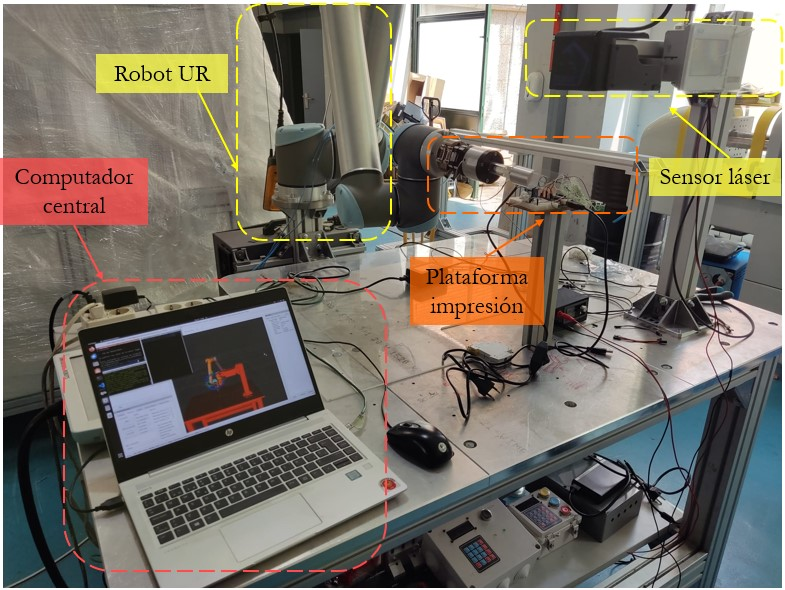
\includegraphics[scale=0.60]{figuras/estacion completa.jpg}
    \caption{Estación robotizada \acrshort{NPAM}}
    \label{fig:estacion completa}
\end{figure}


\section{Líneas futuras}
El trabajo realizado sirve como base para otros proyectos que busquen solventar algunas de las limitaciones antes observadas o implementar nuevas mejoras. Algunas posibles lineas de trabajo futuras pasan por:

\begin{itemize}
    \item Desarrollar un modelo común de cálculo de trayectorias robóticas para procesos \acrshort{NPAM} en base al algoritmo de slicing utilizado. La intención de este proyecto sería implementar sistema de cálculo común que eliminase las diferencias existentes entre las soluciones aportadas por cada uno de los sistemas (slicing y cinemática) empleados en esta arquitectura de control. De este modo se realizaría una potente inversión en la seguridad del entorno de trabajo y en el control que tendría el ingeniero de diseño sobre los movimientos del manipulador robótico.

    \item Implementar un sistema control de velocidad que no dependa exclusivamente de una solución cinemática previa. Esto es, un modelo de cálculo de trayectorias que integre como condiciones de contorno la velocidad máxima de avance en el espacio cartesiano y pudiese compensar automáticamente alinealidades en articulaciones y movimientos ejecutados.

    \item Integrar la estación de fabricación robotizada en un entorno de comunicaciones industriales de mayor complejidad. Un ejemplo de esta propuesta podría ser el conexionado de una estación de cálculo remota que obtuviese las trayectorias por ejecutar y llevase a cabo un análisis en directo de los datos provenientes del proceso de fabricación \acrshort{NPAM}.

    \item Aportar mejoras a la metodología de diseño utilizada enfocadas en que se puede utilizar en diseños de componentes más específicos. Algunos ejemplos pueden ser un regulador de la potencia eléctrica demandada por cada elemento de la instalación asociada a la estación, la implementación de circuitos integrados reguladores de potencia para equipos como la plataforma de impresión o el extrusor; y finalmente un encapsulamiento adecuado para facilitar el uso e instalación de la estación y otros componentes agregables.

    \item Introducir un sistema de aprendizaje híbrido que tome en cuenta la información proveniente del entorno virtual correspondiente al modelo offline y la proveniente del entorno real. Un caso de uso puede ser la introducción de sistemas de visión artificial para calibrar automáticamente la posición de la cama de impresión en la realidad.
\end{itemize}

Pese a su generalidad, todas estas líneas se pueden servir de utilizar los últimos avances en las tecnologías industriales para aumentar su valor añadido como son la inteligencia artificial para labores de diagnóstico de equipos, la compensación de vibraciones mecánicas mediante modelos software, la visión por computador para reconocimiento de errores en piezas o el diseño de materiales para mejorar las propiedades mecánicas del producto deseado.